\begin{figure*}[t]
\centering
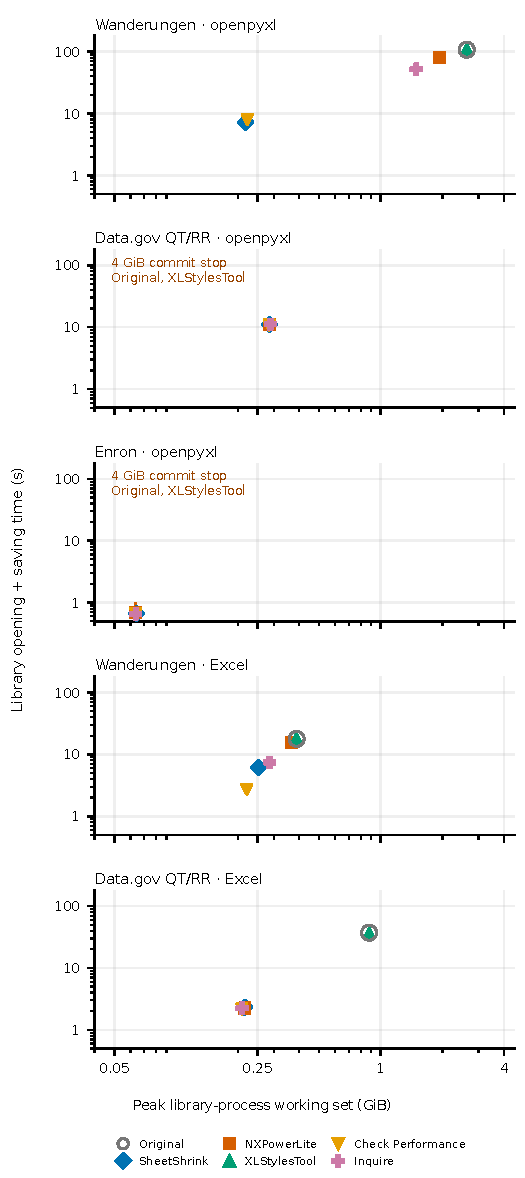
\includegraphics[width=\textwidth]{figures/case-study-resources.pdf}
\caption{Selected open--save endpoints. Points show median library opening plus saving time and the
maximum sampled library-process working set over three attempts; vertical lines
show the observed opening-plus-saving time range. Lower and further left indicate smaller measured cost.
Cleanup time is excluded for every tool. SheetShrink processes a fresh output;
external tools use prepared outputs. Memory covers the Python library worker or
Excel process, excluding cleanup executables and pipeline coordinators.
Excel opening includes application startup and the ownership handshake. Original uses an open circle so
near-overlapping results remain visible. Memory-stop conditions have no completed
time point. Wanderungen and QT/RR use the Ryzen 5 4500U laptop; Enron uses the
Ryzen 7 7800X3D host. Each uses a 4 GiB process-tree commit limit, distinct from
the physical working-set metric on the x-axis. Comparisons are within panels.
Complete library and phase results remain in the artifact.}
\label{fig:case-study-resources}
\end{figure*}
